\documentclass[aps,prl,10pt,onecolumn,superscriptaddress,longbibliography]{revtex4-2}
\usepackage[T1]{fontenc}
\usepackage[utf8]{inputenc}
\usepackage{amsmath,amssymb,bm,graphicx,booktabs}
\usepackage[colorlinks=true,citecolor=blue,urlcolor=blue,linkcolor=blue]{hyperref}
\hypersetup{pdftitle={Supplemental Material: Interlayer-distance control of spectral reconstruction in twisted graphene},pdfauthor={Vladislav Efremkin, Thomas D. Kühne, Emil Prodan}}
\newcommand{\Tr}{\operatorname{Tr}}
\newcommand{\angstrom}{\text{\AA}}
\renewcommand{\theequation}{S\arabic{equation}}
\renewcommand{\thefigure}{S\arabic{figure}}
\renewcommand{\thetable}{S\arabic{table}}
\renewcommand{\thepage}{S\arabic{page}}
\begin{document}
\title{Supplemental Material for\\Interlayer-distance control of spectral reconstruction in twisted graphene}
\author{Vladislav Efremkin}
\affiliation{Center for Advanced Systems Understanding (CASUS), Helmholtz-Zentrum Dresden-Rossendorf (HZDR), 02826 G\"orlitz, Germany}
\author{Thomas D. K\"uhne}
\email{tkuehne@cp2k.org}
\affiliation{Center for Advanced Systems Understanding (CASUS), Helmholtz-Zentrum Dresden-Rossendorf (HZDR), 02826 G\"orlitz, Germany}
\author{Emil Prodan}
\affiliation{Department of Physics, Yeshiva University, New York, New York 10016, USA}
\date{September 16, 2026 --- Author-review draft}
\maketitle

\section{Scope and provenance}

This supplement separates three categories of information: the supplied first-principles DOS images, the calculation settings and geometries directly recoverable from the input files, and a new numerical reproduction of the supplied tight-binding notebook. The principal source is the data package circulated by V. Efremkin on July 23, 2026. It contains ten SZV DOS maps, three DZVP maps, a two-page comparison document, 51 input configurations at $d=2.15\,\angstrom$, and model notebooks. Earlier correspondence documents the construction of the finite upper layer and identifies white columns as calculations that failed to converge. The complete final CP2K output files, state-resolved eigenvalues and projections, and the DFT plotting scripts were not present in that package.

The DFT panels in this draft are the original images. They have not been interpolated, recolored, or used to infer quantitative gap widths. The model panels, by contrast, were regenerated from independently diagonalized Hamiltonians using the stated notebook parameters and an exact change of energy units. Thus the model reproduction is computationally reproducible from the accompanying code, whereas full reproduction of the DFT maps requires the missing state-resolved output and postprocessing. Statements about proposed controls below do not describe calculations already performed.

\section{Atomistic geometry and its limitations}

The supplied $d=2.15\,\angstrom$ series samples $\theta=30^\circ,30.6^\circ,\ldots,60^\circ$. The cell vectors, in angstroms, are
\begin{equation}
 \bm A=(61.4878,0,0),\quad
 \bm B=(30.7439,53.25,0),\quad
 \bm C=(0,0,12.15).
 \label{eq:cell}
\end{equation}
The first 1250 atoms are carbon in the lower layer at $z=0$. They form a $25\times25$ supercell of the two-atom graphene primitive cell. The nearest-neighbor distance is $a_{\rm CC}=1.42\,\angstrom$. The primitive-vector length is $\sqrt{3}a_{\rm CC}$, not $a_{\rm CC}$. The upper sheet is rotated and cut to avoid overlap with its periodic replicas, and its dangling bonds are hydrogen terminated. The supplied C--H distances are approximately $1.09\,\angstrom$. All upper carbon and hydrogen atoms lie at $z=2.15\,\angstrom$.

The finite upper patch contains 955--1013 carbon atoms and 84--100 hydrogen atoms. The total atom count ranges from 2290 to 2362. For example, the $45^\circ$ structure has 984 upper-layer carbon atoms and 94 hydrogen atoms, giving 2328 atoms in total. Figure~\ref{fig:counts} and the accompanying \texttt{data/geometry\_counts.csv} record this variation. An angle scan consequently changes not only registry but also coverage and edge termination. These variations are not equivalent to a twist scan at fixed Hilbert-space dimension in the disk model.

\begin{figure}[h]
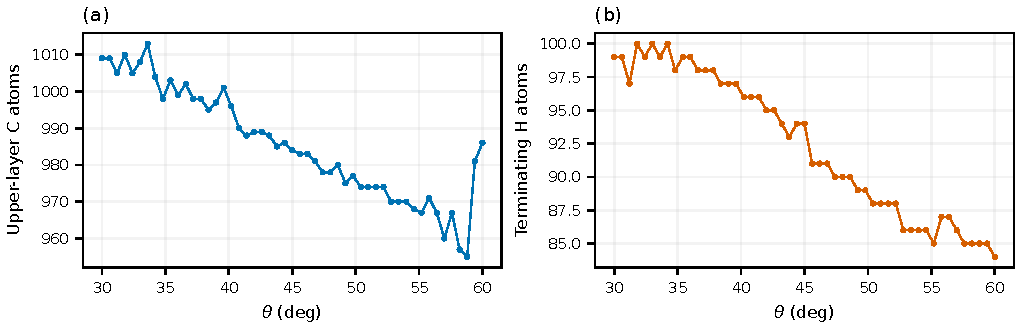
\includegraphics[width=0.88\textwidth]{figures/geometry_counts.pdf}
\caption{Atom counts determined directly from the 51 supplied coordinate files at $d=2.15\,\angstrom$. The lower layer contains 1250 carbon atoms at every angle. Upper-layer carbon and terminating hydrogen counts vary with the construction of the finite patch.}
\label{fig:counts}
\end{figure}

The input specifies periodicity in all three directions. At this separation, the distance from the upper plane to the next lower-layer periodic image along $z$ is $10\,\angstrom$. An isolated-boundary Poisson block is commented out. These facts do not establish convergence with respect to vacuum or electrostatic boundary conditions. The calculation type is \texttt{ENERGY}: neither structural relaxation nor force convergence is demonstrated. An imposed layer separation is not a measured or calculated hydrostatic pressure. In particular, the strongly compressed structures are constrained electronic configurations. Their mechanical stability remains to be tested.

\section{First-principles settings and projected spectral weights}

Table~\ref{tab:settings} summarizes the common input recovered for the 51 configurations. The associated submission script loads a CP2K/2023.1 module, but a program-version header from a completed output is not available. The SZV settings can be audited from the supplied inputs. The precise DZVP basis identifier and all corresponding calculation settings must be confirmed from the separate DZVP runs. Qualitative similarity between their rendered DOS maps does not establish basis convergence.

The inputs specify the libraries \texttt{BASIS\_MOLOPT} and \texttt{GTH\_POTENTIALS}, not the newer UZH parameter files. The UZH protocol~\cite{uzh2026} provides the methodological reference for constructing MOLOPT/GTH parameter sets and separately assessing Gaussian-basis and pseudopotential errors.

\begin{table}[h]
\caption{Settings explicitly present in the supplied $d=2.15\,\angstrom$ inputs. Defaults not specified in those files are not reported as independently verified run parameters.}
\label{tab:settings}
\begin{ruledtabular}
\begin{tabular}{p{0.29\textwidth}p{0.64\textwidth}}
Electronic-structure method & CP2K Quickstep, Gaussian and plane waves (GPW)~\cite{cp2k2020,cp2k2026}, PBE~\cite{pbe1996} \\
Pseudopotentials & GTH-PBE, carbon $q4$, hydrogen $q1$ \\
Gaussian basis & SZV-MOLOPT-GTH for C and H \\
Spin and charge & Spin-polarized, neutral system with multiplicity not explicitly set \\
Density grid & 300-Ry cutoff and five multigrids. Relative cutoff not explicitly set \\
Quickstep accuracy & \texttt{EPS\_DEFAULT} $=10^{-10}$ \\
Self-consistency & \texttt{EPS\_SCF} $=10^{-5}$, maximum 6000 iterations, atomic initial guess \\
Diagonalization and mixing & Standard diagonalization with adaptive threshold 0.01. Broyden mixing with $\alpha=0.2$, buffer 10 \\
Occupation scheme & Fermi--Dirac smearing at 300 K with 300 added molecular orbitals \\
Dispersion & D3 pair-potential input with C9 terms requested and long-range correction disabled~\cite{grimme2010} \\
Reciprocal-space sampling & $\Gamma$-point calculation (no explicit \texttt{KPOINTS} section) \\
DOS output request & \texttt{DELTA\_E} $=0.0001$ in the DOS print block \\
Layer projection & PDOS/LDOS on atoms 1--1250 with component output requested \\
Boundary and run type & Fixed-geometry \texttt{ENERGY} run with cell periodicity XYZ
\end{tabular}
\end{ruledtabular}
\end{table}

The D3 term accounts for dispersion interactions that are important for interlayer binding in graphene and for its equilibrium layer separation~\cite{lebedeva2017}. It depends on the geometry and is added to the DFT energy and forces. It does not by itself alter the Kohn--Sham potential at a fixed geometry. Dispersion could affect the spectrum indirectly through a relaxed structure, but such relaxation is not part of the supplied input series.

Let $\{\chi_\mu\}$ be the nonorthogonal Gaussian basis. The matrices
\begin{equation}
 H_{\mu\nu,\sigma}=\langle\chi_\mu|\hat H_{\rm KS,\sigma}|\chi_\nu\rangle,
 \qquad S_{\mu\nu}=\langle\chi_\mu|\chi_\nu\rangle
\end{equation}
represent the Kohn--Sham operator and the basis overlap. They satisfy
\begin{equation}
 \bm H_\sigma\bm c_{n\sigma}=\varepsilon_{n\sigma}\bm S\bm c_{n\sigma},
 \qquad \bm c_{n\sigma}^{\dagger}\bm S\bm c_{m\sigma}=\delta_{nm}.
\end{equation}
For a positive-definite overlap matrix, symmetric orthogonalization~\cite{lowdin1950} gives
\begin{equation}
 \widetilde{\bm H}_\sigma=\bm S^{-1/2}\bm H_\sigma\bm S^{-1/2},
 \qquad \widetilde{\bm c}_{n\sigma}=\bm S^{1/2}\bm c_{n\sigma}.
\end{equation}
The CP2K 2023.1 PDOS implementation uses the corresponding L\"owdin-type coefficients. If $\bm\Pi_L$ selects orthogonalized orbital labels belonging to the lower layer, then
\begin{equation}
 w^{(L)}_{n\sigma}=\widetilde{\bm c}_{n\sigma}^{\dagger}\bm\Pi_L
 \widetilde{\bm c}_{n\sigma},\qquad 0\leq w^{(L)}_{n\sigma}\leq1.
\end{equation}
This is an orbital-partition weight, not a real-space integral over a geometrical slab. Summing over a complete partition of all orbital labels recovers unit weight for each normalized state. A single-layer projection need not do so. Consequently, suppressed projected weight need not imply an absence of eigenvalues in the whole system.

A $\Gamma$-point supercell spectrum consists of discrete eigenvalues. Broadening it is not equivalent to a converged Brillouin-zone integration. In an unrotated $N\times N$ graphene cell, primitive-cell $K$ folds to the supercell $\Gamma$ only if $N$ is divisible by three. The present $N=25$ does not satisfy that condition. A Dirac cone therefore cannot be diagnosed from a $\Gamma$-only angle--DOS map. Its horizontal coordinate is twist angle, not wave vector.

Several distinctions matter for reproducibility. The 300-K Fermi--Dirac temperature sets occupations, whereas a Gaussian DOS width sets display broadening. The DOS print grid spacing is not automatically the postprocessing Gaussian width. Adding 300 molecular orbitals to the SCF diagonalization also does not by itself establish which unoccupied orbitals were written to every PDOS output. That requires the print settings and actual output. The supplied panels label their ordinate $E-E_F$ but do not explicitly print an energy unit or a calibrated color bar. Their original scale is retained here. Confirmation of the energy conversion, spin summation, normalization, broadening, and printed virtual-state range is needed before numerical gap widths can be reported in electronvolts. Separately shifting each configuration by its own $E_F$ can further obscure absolute spectral shifts.

\section{Tight-binding model and the small-energy-scale issue}

The model starts from a honeycomb point set
\begin{equation}
 P_R=\left\{n_1\bm a_1+n_2\bm a_2+\bm b_s:
 |n_1\bm a_1+n_2\bm a_2+\bm b_s|\leq R\right\},
\end{equation}
where $\bm a_1=(\sqrt3a,0)$, $\bm a_2=(\sqrt3a/2,3a/2)$, and $\bm b_s\in\{(0,0),(0,a)\}$. The two-layer set is
\begin{equation}
 X_{\theta,d}=\{(\bm r,0):\bm r\in P_R\}\cup
              \{(\mathsf R_\theta\bm r,d):\bm r\in P_R\}.
\end{equation}
Here $\mathsf R_\theta$ is a coordinate rotation matrix, not a Hilbert-space Hamiltonian. The operator $\hat H$ acts on orthonormal site states. Its matrix elements are
\begin{equation}
 H_{ij}=\begin{cases}
 t_0\exp(-|\bm x_i-\bm x_j|/\xi),&i\ne j,\\
 0,&i=j.
 \end{cases}
 \label{eq:model}
\end{equation}
All pairs are retained. The supplied notebook uses $t_0=1$ in arbitrary energy units, with positive real hopping. There is no magnetic Peierls phase, orbital-angular factor, or fit to a carbon $p_z$ Hamiltonian. Same-sublattice further-neighbor hopping is present. Zero on-site energy implies $\Tr\bm H=0$, but not exact particle--hole symmetry. Zero energy is not automatically the half-filling chemical potential.

For $a=1$ and $\xi=0.03$, the nearest-neighbor intralayer hopping is
\begin{equation}
 t_{\rm nn}=t_0e^{-a/\xi}
            =3.33824\times10^{-15}t_0.
 \label{eq:small}
\end{equation}
This explains energies of order $10^{-14}t_0$ in the original plots and reciprocal DOS scales of order $10^{14}/t_0$. Such values are not floating-point underflow. They do, however, obscure the natural model units and cannot be interpreted as physical electronvolt energies without calibration. The exact dimensionless Hamiltonian is
\begin{equation}
 \overline H_{ij}=\frac{H_{ij}}{t_{\rm nn}}
 =\exp\!\left[\frac{a-|\bm x_i-\bm x_j|}{\xi}\right]\quad(i\ne j),
 \qquad \overline H_{ii}=0.
 \label{eq:rescale}
\end{equation}
Eigenvectors are unchanged, and $\epsilon_n=E_n/t_{\rm nn}$. This rescaling preserves all dimensionless spectral gaps and does not alter the physical content of the specified model.

The DOS must be transformed with the same change of variables. For a DOS $\rho(E)$ normalized to one state, probability conservation gives
\begin{equation}
 \overline\rho(\epsilon)\,d\epsilon=\rho(E)\,dE,
 \qquad \overline\rho(\epsilon)=t_{\rm nn}\rho(t_{\rm nn}\epsilon),
 \qquad \overline\eta=\eta/t_{\rm nn}.
 \label{eq:jacobian}
\end{equation}
Multiplying only the energy axis, while leaving the DOS and broadening unchanged, would therefore be inconsistent. The independently regenerated figures use Eqs.~\eqref{eq:rescale} and \eqref{eq:jacobian} throughout.

The strongest allowed interlayer matrix element is that for vertical alignment. Its ratio to the intralayer nearest-neighbor hopping is
\begin{equation}
 t_\perp^{\max}/t_{\rm nn}=e^{(a-d)/\xi}.
\end{equation}
At $\xi/a=0.03$, the values for $d/a=0.99,0.98,0.97$ are respectively 1.396, 1.948, and 2.718. This ratio changes under a change of distance and cannot be removed by a global energy rescaling. Likewise, changing $\xi$ changes the intralayer range, for example
\begin{equation}
 t_{\rm next}/t_{\rm nn}=e^{-(\sqrt3-1)a/\xi}.
\end{equation}
The $\xi/a=0.03,0.1,0.3$ comparison is thus a family of different Hamiltonians, not merely three choices of units. Assigning a conventional graphene hopping in electronvolts would still leave the interlayer angular dependence, distance law, sign convention, and chemical validity uncalibrated. The model's $d/a\simeq1$ is not a prediction that real graphene should be compressed to its C--C bond length.

\section{Independent numerical reproduction}

The reproduced model uses $R/a=25$, giving 1510 sites in each layer and a $3020\times3020$ real-symmetric matrix. The earlier notebook example used a larger radius. It must not be confused with the latest parameter series. We evaluated all eigenvalues at 41 equally spaced angles from $0$ to $\pi/3$, inclusive, for five parameter combinations: $(d/a,\xi/a)=(0.99,0.03),(0.98,0.03),(0.97,0.03),(0.97,0.1),(0.97,0.3)$.

The spectra at negative angles follow exactly from those at positive angles. Exchanging the two identical layers, applying a rigid in-plane rotation by $-\theta$, and reflecting the normal coordinate maps the pair $(P_R,\mathsf R_\theta P_R)$ to $(P_R,\mathsf R_{-\theta}P_R)$ up to relabeling. Pair distances are unchanged, so the Hamiltonians are related by a permutation and have identical eigenvalues. This gives an 81-angle display on $[-60^\circ,60^\circ]$. It does not establish exact $60^\circ$ periodicity of the finite site-centered disk: a honeycomb lattice centered on a carbon site has a different finite-boundary symmetry from one centered on a hexagon. Nor does it justify imposing a bulk periodicity on the angle-dependent DFT patches.

The plotted model DOS is
\begin{equation}
 \overline\rho_{\overline\eta}(\epsilon;\theta)
 =\frac{1}{N}\sum_{n=1}^N
 \frac{\exp[-(\epsilon-\epsilon_n(\theta))^2/(2\overline\eta^2)]}
 {\sqrt{2\pi}\,\overline\eta},\qquad N=3020.
\end{equation}
Its integral over the entire real axis is one, not the unnormalized total number of states. Following the notebook convention, each parameter set uses the global spectral span over all sampled angles divided by 1000 as its Gaussian width. The width can therefore differ between panels. The original 500-point display grid had a spacing of about twice this width. We use 2001 points, approximately half the width, to sample the same kernel more smoothly. This improves rendering, not the underlying physical resolution. The common color scale is clipped above $\overline\rho=0.5$ to reveal weaker structures. The plotted energy window is $[-6,6]$ in units of $t_{\rm nn}$.

The source package contains \texttt{analysis/reproduce\_tb.py}, \texttt{analysis/make\_figures.py}, and the eigenvalue arrays in \texttt{data/tb\_reproduction}. The first script constructs the normalized Hamiltonian directly and diagonalizes it with SciPy. The second computes the Gaussian DOS and assembles the figures. These are independent finite-size reproductions of the notebook model, not a new DFT calculation, a thermodynamic-limit extrapolation, or a computation of topological invariants.

\section{What would establish a topological gap?}

The acoustic experiment motivating this study combined spectral measurements with boundary-state evolution under a controllable phason~\cite{ni2019}. Twisted mechanical bilayers supplied a more direct setting in which incommensurate geometry organizes gaps through higher-dimensional topology~\cite{rosa2021}. Neither precedent establishes topology from the appearance of a DOS image alone. A two-dimensional bilayer has two relative-translation coordinates, providing a natural phason torus. These coordinates are distinct from the twist angle. Sliding responses and bilayer gap-labeling frameworks make that distinction explicit~\cite{su2020,fujimoto2020,yoshii2023}.

For a bulk operator, the integrated DOS is defined using a trace per volume,
\begin{equation}
 \mathcal N(E;\theta)=\tau\bigl[\mathbf1_{(-\infty,E]}(\hat H_\theta)\bigr].
\end{equation}
The normalization of $\tau$ must be fixed before a gap label is compared across geometries. An integral of lower-layer PDOS generally does not equal this trace: it measures projected spectral weight rather than the rank density of a bulk spectral projector. A finite matrix also has discrete spacings between eigenvalues, many of which need not survive as bulk gaps.

In the noncommutative-torus construction of Ref.~\cite{rosa2021}, a gap's integrated density is constrained by integer coefficients and entries of a $2\times2$ geometric matrix $A$. In that work's notation and sign convention, the trace takes the form
\begin{equation}
 \mathcal N(G)=n_{\varnothing}+n_{\{1,3\}}A_{11}
 +n_{\{1,4\}}A_{12}+n_{\{2,3\}}A_{21}
 +n_{\{2,4\}}A_{22}+n_{\{1,2,3,4\}}\det A.
\end{equation}
The two-index and four-index integer labels refer to the four-dimensional algebra, whereas the indices of $A$ refer to the two-dimensional lattice geometry. This expression is framework- and normalization-dependent, not a universal fitting formula for the supplied CP2K maps. Moreover, if the geometric family has $\det A=1$, its trace constrains the constant combination $n_{\varnothing}+n_{\{1,2,3,4\}}$ rather than separately identifying the second-Chern coefficient. A spectral fit along that family alone therefore cannot provide a unique second-Chern assignment.

Establishing the proposed connection requires candidate gaps that survive size, boundary, reciprocal-space, and numerical convergence tests, followed by a justified gap-label or phason-response calculation for the corresponding bulk projector. No such label, Chern number, quantized pump, or physical Hall response is reported here. The real hopping Hamiltonian carries no magnetic flux. Synthetic-dimensional topology must not be conflated with the magnetic Hofstadter mechanism.

\section{Matched references and outstanding controls}

An especially useful next calculation is a matched noninteracting-layer reference. With a common energy origin and identical broadening, define the unnormalized total-DOS change as
\begin{equation}
 \Delta D(E;\theta,d)=D_{\rm bilayer}(E;\theta,d)
                    -D_1^{\rm ref}(E;\theta)-D_2^{\rm ref}(E;\theta).
 \label{eq:delta}
\end{equation}
The references retain the actual layer geometries and edge termination but remove their mutual interaction. The simplification $D_1^{\rm ref}+D_2^{\rm ref}=2D_{\rm mono}$ is valid only for equivalent layers with the same state-count normalization. For the identical model disks, if every DOS is instead normalized per state, the noninteracting reference is one monolayer DOS, not twice that DOS. In the DFT geometry the layers are inequivalent, so a periodic carbon sheet and the actual hydrogen-terminated patch must be treated separately. A consistent basis-space convention is also necessary if basis-set-superposition effects are to be separated.

Separately setting each reference's Fermi energy to zero is not a common energy alignment. A vacuum or other well-defined electrostatic reference is needed for quantitative DFT differences. When the same complete state space and normalization are used, the integral of the unnormalized $\Delta D$ over all energies vanishes: coupling redistributes states rather than creating them. A restricted occupied-state or printed-orbital window need not satisfy this sum rule. The matched-reference calculation was proposed in the earlier analysis but is not included among the supplied results.

Other outstanding controls are: completed SCF output for every column; spin and occupation checks; the printed unoccupied-state range; larger Gaussian bases and grid cutoffs; reciprocal-space sampling; vacuum convergence; larger upper patches and interior-only projections; a fixed-boundary or coverage-controlled angle series; and relaxation or force analysis of the compressed structures. In the model, radius and broadening series are needed before low-DOS regions are called bulk gaps. These tests should precede numerical gap widths, critical distances, pressure assignments, or topological labels.

\clearpage
\section{Complete first-principles image survey}
\begin{figure}[h]
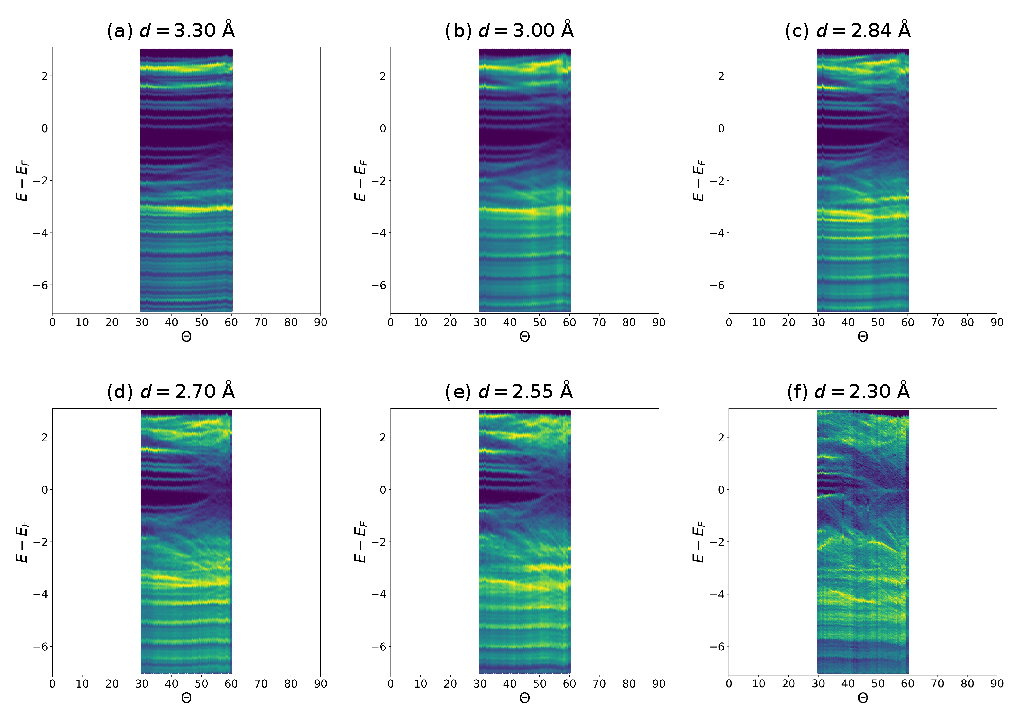
\includegraphics[width=\textwidth]{figures/dft_survey_1.pdf}
\caption{Original SZV lower-layer projected DOS panels for $d=3.30$, $3.00$, $2.85$, $2.70$, $2.55$, and $2.30\,\angstrom$. Axes, colors, and missing columns are preserved. The displayed ordinate is the original $E-E_F$ scale. No calibrated common color scale is asserted. The full angular axes should not be mistaken for a larger sampled interval.}
\end{figure}

\clearpage
\begin{figure}[t]
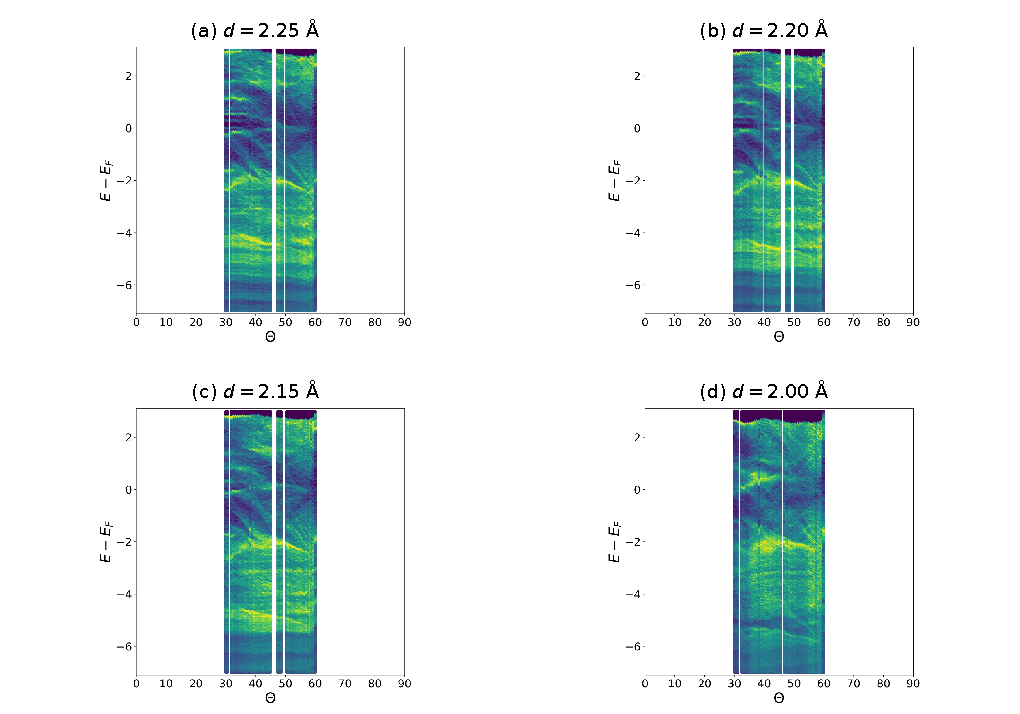
\includegraphics[width=0.88\textwidth]{figures/dft_survey_2.pdf}
\caption{Original SZV lower-layer projected DOS panels for $d=2.25$, $2.20$, $2.15$, and $2.00\,\angstrom$. A missing white column is not a gap. A dark region can reflect small layer weight, broadening, or finite-size discreteness and is not by itself a bulk spectral gap.}
\end{figure}

\clearpage
\begin{figure}[t]
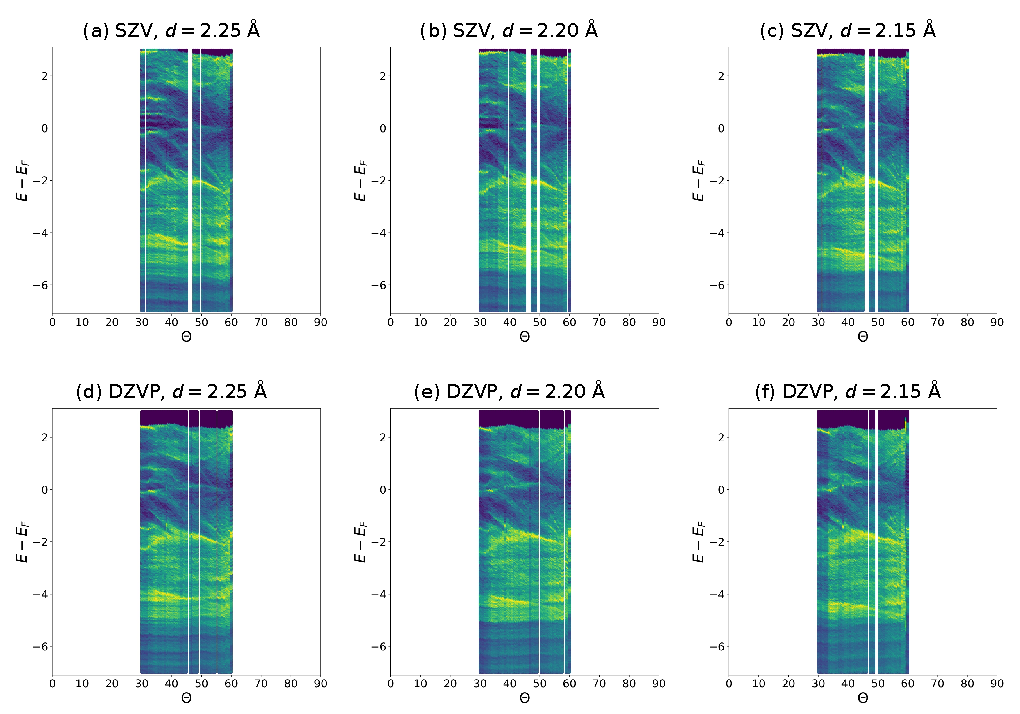
\includegraphics[width=\textwidth]{figures/basis_comparison.pdf}
\caption{Original SZV (top) and DZVP (bottom) panels at $d=2.25$, $2.20$, and $2.15\,\angstrom$. Related large-scale structures provide a qualitative basis check. The source images do not establish a matched quantitative intensity normalization, converged gap width, or a complete basis-convergence series.}
\end{figure}

\clearpage
\section{Dependence on the model hopping range}
\begin{figure}[h]
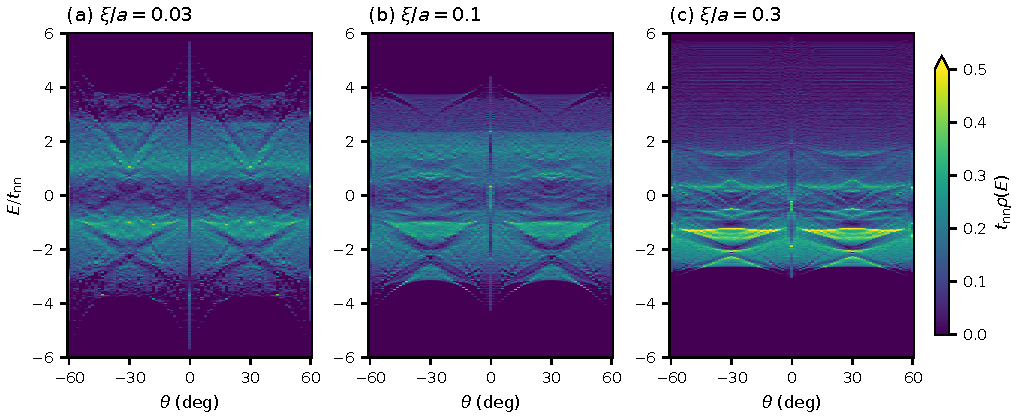
\includegraphics[width=\textwidth]{figures/tb_range.pdf}
\caption{Independently reproduced model DOS at fixed $R/a=25$ and $d/a=0.97$, for $\xi/a=0.03$, $0.1$, and $0.3$. Each Hamiltonian is normalized by its own nearest-neighbor intralayer hopping. Changing $\xi$ changes both the relative interlayer coupling and further-neighbor intralayer hopping. Broadening follows the spectral-span convention described above. The common intensity scale is clipped above 0.5.}
\end{figure}

\makeatletter
\immediate\write\@auxout{\string\citation{bibliography_control}}
\makeatother
\bibliographystyle{apsrev4-2}
\bibliography{references}
\end{document}
